\documentclass[11pt]{article}

\usepackage[margin=1in]{geometry}
\usepackage{booktabs}
\usepackage{graphicx}
\usepackage{hyperref}
\usepackage{amsmath}
\usepackage{amssymb}
\usepackage{xcolor}
\usepackage{enumitem}
\usepackage{listings}
\usepackage{caption}
\usepackage{subcaption}
\usepackage{natbib}
\usepackage{tikz}
\usetikzlibrary{arrows.meta, positioning, calc}

\hypersetup{colorlinks=true, linkcolor=blue, citecolor=blue, urlcolor=blue}
\emergencystretch=1em   % allow slightly stretched whitespace to avoid overflow from long citations

\lstset{
  language=Python,
  basicstyle=\ttfamily\small,
  keywordstyle=\color{blue},
  commentstyle=\color{gray},
  stringstyle=\color{red!60!black},
  showstringspaces=false,
  frame=single,
  breaklines=true,
  columns=fullflexible,
}

\title{\textbf{reptimeline}: Tracking Discrete Representation Evolution\\During Neural Network Training}

\author{J. Arturo Ornelas Brand\\
Independent Researcher\\
\texttt{arturoornelas62@gmail.com}\\
\url{https://github.com/arturoornelasb/reptimeline}
}

\date{March 2026}

\begin{document}
\maketitle

\begin{abstract}
We present \textbf{reptimeline}, a Python library for tracking how discrete representations evolve during neural network training. Unlike scalar logging tools (WandB, TensorBoard) that report aggregate metrics, reptimeline tracks per-code lifecycle events: when concepts become distinguishable (births), when representations collapse (deaths), when relationships form between concept pairs (connections), and where phase transitions occur in training dynamics. The library additionally discovers what each code element encodes---anti-correlated pairs, dependency chains, and three-way AND-gate interactions---without requiring prior ontological knowledge, with all discoveries subjected to multiple-comparison correction (Bonferroni or Benjamini-Hochberg FDR). Causal verification uses bootstrap confidence intervals, permutation tests, and Cohen's $d$ effect sizes. reptimeline ships three built-in extractors (VQ-VAE, SAE, FSQ), five static and four interactive visualizations, JSON/CSV export, and a command-line interface. We validate on three architecturally distinct backends: a 32-bit binary autoencoder on MNIST (decoder determinism verified: 100\%), sparse autoencoder features on Pythia-70M (8/16 features with finite KL selectivity, mean 26.8$\times$ L2 ratio with bootstrap 95\% CI, plus 8 features with zero cross-activation attributable to SAE sparsity), and a 63-bit neurosymbolic projection head (crystallization event invisible to loss curves). reptimeline is the only tool that combines lifecycle tracking, bottom-up feature discovery, auto-labeling, causal verification, and theory reconciliation in a single backend-agnostic package. Available via \texttt{pip install reptimeline} under BUSL-1.1.
\end{abstract}


% ============================================================
\section{Introduction}
\label{sec:intro}
% ============================================================

Every system that quantizes neural representations into discrete codes---VQ-VAE codebooks \citep{vandenoord2017neural}, finite scalar quantization \citep{mentzer2024finite}, sparse auto\-encoders \citep{cunningham2023sparse, sharkey2022taking, bricken2023monosemanticity}, concept bottleneck models \citep{koh2020concept}, or binary autoencoders---faces the same blind spot: \emph{you can see what the codes look like after training, but not how they got there.}

Current monitoring tools log scalar aggregates: codebook utilization, perplexity, reconstruction loss. These tell practitioners \emph{that} something changed, not \emph{what} changed. When codebook collapse occurs at step~27{,}500, a loss curve shows a kink. But which codes died? Did they die together? Was there a phase transition? Which concepts lost their unique representations? These questions require per-code temporal analysis that no existing tool provides.

\textbf{reptimeline} fills this gap. Given a sequence of model checkpoints and a set of probe concepts, it:
\begin{enumerate}[nosep]
    \item \textbf{Tracks} per-code lifecycle events (births, deaths, connections, phase transitions) and per-bit stability scores;
    \item \textbf{Discovers} what each code element encodes (duals, dependencies, 3-way interactions) with statistical correction (Bonferroni, BH-FDR);
    \item \textbf{Labels} discovered features automatically (embedding centroid, contrastive, or LLM);
    \item \textbf{Verifies} that discovered features are causal via intervention experiments with bootstrap CIs, permutation tests, and effect sizes;
    \item \textbf{Reconciles} discovered structure against a theoretical ontology and suggests corrections in both directions.
\end{enumerate}

Critically, reptimeline is \emph{backend-agnostic}: it operates on any system that produces a mapping from concepts to discrete code vectors. We validate this claim on three architecturally distinct backends (Section~\ref{sec:cases}).


% ============================================================
\section{Design and Architecture}
\label{sec:design}
% ============================================================

\subsection{Pipeline Overview}

Figure~\ref{fig:architecture} shows the reptimeline pipeline. The user either implements a single abstract class (\texttt{RepresentationExtractor}) or uses one of the three built-in extractors (Section~\ref{sec:extractors}) to load a checkpoint and return discrete codes for a set of probe concepts. Everything downstream is backend-agnostic.

\begin{figure}[ht]
\centering
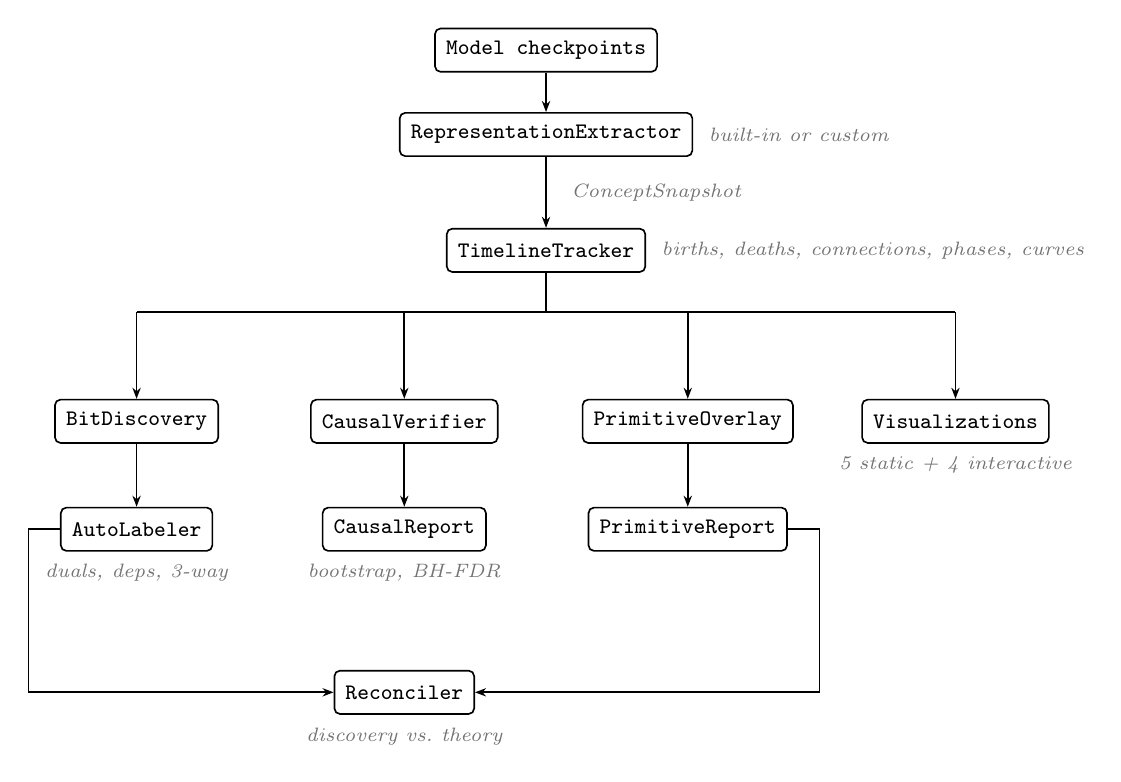
\begin{tikzpicture}[
  box/.style={draw, rounded corners=2pt, font=\footnotesize\ttfamily,
              minimum height=5.5mm, inner xsep=4pt, inner ysep=2pt},
  note/.style={font=\scriptsize\itshape, text=black!55},
  >={Stealth[length=4pt]},
  semithick,
  node distance=5mm
]

% --- Vertical spine ---
\node[box] (ckpt) {Model checkpoints};
\node[box, below=of ckpt] (ext) {RepresentationExtractor};
\node[box, below=9mm of ext] (tt) {TimelineTracker};

% --- Four branches (wide spread) ---
\node[box, below=16mm of tt, xshift=-52mm] (bd) {BitDiscovery};
\node[box, below=16mm of tt, xshift=-18mm] (cv) {CausalVerifier};
\node[box, below=16mm of tt, xshift=18mm]  (po) {PrimitiveOverlay};
\node[box, below=16mm of tt, xshift=52mm]  (viz) {Visualizations};

% --- Second level ---
\node[box, below=8mm of bd] (al) {AutoLabeler};
\node[box, below=8mm of cv] (cr) {CausalReport};
\node[box, below=8mm of po] (pr) {PrimitiveReport};

% --- Bottom ---
\node[box, below=15mm of cr, xshift=0mm] (rec) {Reconciler};

% === Arrows: spine ===
\draw[->] (ckpt) -- (ext);
\draw[->] (ext) -- (tt);

% === Arrows: horizontal bar then down to branches ===
\coordinate (bar) at ($(tt.south)+(0,-5mm)$);
\draw (tt.south) -- (bar);
\draw (bar -| bd.north) -- (bar -| viz.north);
\draw[->] (bar -| bd.north) -- (bd.north);
\draw[->] (bar -| cv.north) -- (cv.north);
\draw[->] (bar -| po.north) -- (po.north);
\draw[->] (bar -| viz.north) -- (viz.north);

% === Arrows: second level ===
\draw[->] (bd) -- (al);
\draw[->] (cv) -- (cr);
\draw[->] (po) -- (pr);

% === Arrows: to Reconciler (exit sideways to avoid annotations) ===
\draw[->] (al.west) -- ++(-4mm,0) |- (rec.west);
\draw[->] (pr.east) -- ++(4mm,0) |- (rec.east);

% === Annotations ===
\node[note, right=2pt of ext] {built-in or custom};
\node[note] at ($(ext.south)!0.5!(tt.north) + (14mm,0)$) {ConceptSnapshot};
\node[note, right=2pt of tt] {births, deaths, connections, phases, curves};
\node[note, below=1pt of viz] {5 static + 4 interactive};
\node[note, below=1pt of al] {duals, deps, 3-way};
\node[note, below=1pt of cr] {bootstrap, BH-FDR};
\node[note, below=1pt of rec] {discovery vs.\ theory};

\end{tikzpicture}
\caption{reptimeline pipeline. The user provides only the extractor (or uses a built-in one for VQ-VAE, SAE, or FSQ); all downstream modules are backend-agnostic.}
\label{fig:architecture}
\end{figure}

\subsection{Core Data Structure}

The universal exchange format is \texttt{ConceptSnapshot}:

\begin{lstlisting}
ConceptSnapshot(
    step=27500,          # training step
    codes={              # concept -> discrete code
        "king":  [1, 0, 1, 1, 0, ...],
        "queen": [1, 0, 1, 0, 1, ...],
        ...
    },
    continuous={...},    # optional: continuous embeddings
    metadata={...}       # optional: backend-specific info
)
\end{lstlisting}

This minimal interface---a step number and a dictionary mapping concept names to integer lists---is sufficient to support VQ-VAE codebook indices, SAE binarized activations, binary autoencoder outputs, triadic bit projections, and any future discrete representation scheme. An optional \texttt{continuous} field allows hybrid discrete+continuous analysis, and \texttt{metadata} stores backend-specific information (e.g., codebook size, SAE top-$k$).

\subsection{Built-in Extractors}
\label{sec:extractors}

While users can implement the \texttt{RepresentationExtractor} abstract base class for any model, reptimeline ships three ready-to-use extractors:

\begin{itemize}[nosep]
    \item \textbf{VQVAEExtractor}: converts VQ-VAE codebook indices into binary indicator vectors (one-hot over the codebook). Similarity via Jaccard index.
    \item \textbf{SAEExtractor}: binarizes sparse autoencoder activations via top-$k$ selection.
    Includes a built-in intervention helper (\texttt{make\_inter\-vene\_fn}) for zero-ablation causal testing: zero a feature in SAE space, decode back, and measure reconstruction change.
    Supports optional feature-index mapping for tracking subsets of large dictionaries (e.g., 256 out of 32K features).
    \item \textbf{FSQExtractor}: handles Finite Scalar Quantization~\citep{mentzer2024finite} with two binarization modes: \emph{nonzero} (1 if level $\neq 0$, one bit per dimension) and \emph{onehot} (full one-hot per dimension, total bits $= \sum n_{\text{levels}}$). Supports multi-quantizer architectures.
\end{itemize}

All three extractors inherit automatic checkpoint discovery that parses common naming conventions (\texttt{model\_step*.pt}, \texttt{checkpoint-*.pt}, \texttt{step\_*.safe\-tensors}) and batch extraction with progress bars.


\subsection{Timeline Analysis}

\texttt{TimelineTracker} consumes a sequence of snapshots and computes:

\begin{itemize}[nosep]
    \item \textbf{Births}: first step where concept $c$ has bit $b$ active (and it persists).
    \item \textbf{Deaths}: step where bit $b$ becomes permanently inactive for concept $c$.
    \item \textbf{Connections}: step where concepts $c_1, c_2$ first share a code element.
    \item \textbf{Curves}: per-step entropy (mean binary entropy across all code elements), churn rate (fraction of concepts whose code changed from the previous step), and utilization (ratio of unique codes to total concepts---closer to 1 means more discriminative).
    \item \textbf{Stability}: per-bit stability scores in $[0, 1]$, measuring the fraction of (concept, step) pairs where a bit remained unchanged from the prior checkpoint.
    \item \textbf{Phase transitions}: detected via statistical change-point analysis---a transition is flagged when $|\Delta_t| > \mu + 2\sigma$ for any curve.
\end{itemize}

\subsection{Feature Discovery}

\texttt{BitDiscovery} analyzes a single snapshot to discover structure without prior ontological knowledge:

\begin{itemize}[nosep]
    \item \textbf{Duals}: pairs $(b_i, b_j)$ with Pearson correlation $< -0.3$ across concepts. These are anti-correlated features---when one is active, the other tends to be inactive.
    \item \textbf{Dependencies}: directed edges $b_p \to b_c$ where $P(b_p = 1 \mid b_c = 1) \geq 0.9$.
    \item \textbf{Three-way AND-gates}: triples $(b_i, b_j, b_r)$ where $P(b_r = 1 \mid b_i = 1 \wedge b_j = 1) \geq \tau$ but $\max(P(b_r \mid b_i), P(b_r \mid b_j)) < \tau$, with $\tau = 0.7$ by default. Additionally, the interaction strength $P(b_r \mid b_i, b_j) - \max(P(b_r \mid b_i), P(b_r \mid b_j))$ must exceed a minimum threshold (default $0.2$). These represent features that activate \emph{only} when two other features are jointly active. Complexity is $O(K^3)$ where $K$ is the number of active bits; in practice $K < 100$ and discovery completes in seconds.
    \item \textbf{Hierarchy}: bits ordered by stabilization step---the training step at which a bit's activation pattern stops changing across consecutive checkpoints.
\end{itemize}

All discovery methods apply multiple-comparison correction: Bonferroni correction for duals and dependencies, and Benjamini-Hochberg FDR correction (via 200-permutation $p$-values per candidate) for triadic interactions. A \texttt{null\_baseline()} method generates random codes to estimate false-positive rates under the null hypothesis.

\subsection{Auto-Labeling and Reconciliation}

\texttt{AutoLabeler} translates discovered bit patterns into human-readable labels via three strategies: (1)~\emph{embedding centroid}---find the word whose embedding is closest to the centroid of active concepts; (2)~\emph{contrastive}---find the word that best separates active from inactive concepts in embedding space (direction vector: $\mathbf{c}_{\text{active}} - \mathbf{c}_{\text{inactive}}$); (3)~\emph{LLM}---ask a language model ``what do these concepts have in common?'' Labels can be exported as a \texttt{primitivos.json} file via \texttt{export\_as\_primitives()}, closing the loop from discovery back to overlay analysis.

\texttt{Reconciler} compares discovered structure against a theoretical ontology (\texttt{PrimitiveOverlay}) and classifies mismatches by type and severity:
\begin{itemize}[nosep]
    \item \textbf{Bit mismatches}: \emph{dead\_but\_assigned} (critical---primitive's bit never activates), \emph{active\_but\_un\-assigned} (warning---active bit has no primitive), \emph{semantic\_drift} (info---bit too broadly active).
    \item \textbf{Dual mismatches}: anti-correlated pairs present in theory but absent in model (or vice versa).
    \item \textbf{Dependency mismatches}: required parent$\to$child edges absent in model or discovered edges absent in theory.
\end{itemize}
An \emph{agreement score} quantifies overall alignment: $1 - (\text{critical mismatches} / n_{\text{primitives}})$. The Reconciler produces correction suggestions in \emph{both directions}: to the model's training anchors (how to retrain) and to the theory (how to update \texttt{primitivos.json}).

\subsection{Causal Verification}

\texttt{CausalVerifier} tests whether discovered features have selective causal effects. The user provides an intervention function $f(c, b) \to \mathbb{R}$ that returns the effect of ablating bit $b$ for concept $c$ (e.g., L2 reconstruction change or KL divergence). For each tested bit:

\begin{enumerate}[nosep]
    \item Concepts are partitioned into \emph{labeled} (bit $= 1$) and \emph{other} (bit $= 0$) groups.
    \item The intervention function is called for all concepts.
    \item A \textbf{bootstrap confidence interval} (default 1{,}000 resamples) is computed on the selectivity ratio: $\bar{f}_{\text{labeled}} / \bar{f}_{\text{other}}$.
    \item A two-sided \textbf{permutation test} (default 1{,}000 permutations) yields a $p$-value.
    \item \textbf{Cohen's $d$} measures effect size between groups.
    \item \textbf{Benjamini-Hochberg FDR correction} is applied across all tested bits at $\alpha = 0.05$.
\end{enumerate}

A bit is considered causally selective if it is significant after FDR correction \emph{and} its selectivity ratio exceeds a threshold (default $1.5\times$). The overall verdict is \emph{causal\_evidence\_found} if at least 3 bits meet both criteria. All statistical functions (\texttt{bootstrap\_ci}, \texttt{permutation\_test}, \texttt{benjamini\_hochberg}, \texttt{effect\_size\_cohens\_d}) are implemented in \texttt{stats.py} using only NumPy, with no SciPy dependency.

\subsection{Visualization and CLI}

reptimeline provides five static visualizations (matplotlib):
\begin{enumerate}[nosep]
    \item \textbf{Phase dashboard}: three-panel plot of entropy, churn, and utilization curves with phase transitions marked as vertical lines.
    \item \textbf{Swimlane}: per-concept heatmap where rows are concepts, columns are training steps, and cells show bit activation state (Figure~\ref{fig:swimlane}).
    \item \textbf{Churn heatmap}: per-bit churn rates across training, highlighting the least stable bits.
    \item \textbf{Layer emergence}: horizontal bar chart showing when each layer's primitives first stabilize.
    \item \textbf{Causal heatmap}: selectivity ratio per bit with bootstrap confidence intervals as error bars.
\end{enumerate}
Four of these (phase dashboard, swimlane, causal heatmap, churn heatmap) also have interactive Plotly versions with hover details and zoom, available when Plotly is installed.

\textbf{Export.} \texttt{Timeline} supports \texttt{save\_json()} / \texttt{load\_json()} for persistence and \texttt{to\_csv()} for exporting five CSV files: events, connections, curves, stability, and codes.

\textbf{CLI.} The command-line interface provides access to the full pipeline:
\begin{verbatim}
reptimeline --snapshots data.json --discover --plot
reptimeline --snapshots data.json --overlay primitivos.json
reptimeline --snapshots data.json --causal effects.json --output results.json
\end{verbatim}


% ============================================================
\section{Case Studies}
\label{sec:cases}
% ============================================================

We validate reptimeline on three backends spanning supervised image models, unsupervised LLM internals, and end-to-end neurosymbolic systems. Table~\ref{tab:results} summarizes the results.

\begin{table}[h]
\centering
\caption{reptimeline analysis across three backends. All numbers are from production runs, not toy examples.}
\label{tab:results}
\small
\begin{tabular}{lccc}
\toprule
& \textbf{MNIST BAE} & \textbf{Pythia SAE} & \textbf{TriadicGPT} \\
\midrule
Architecture & Binary AE (32-bit) & SAE on Pythia-70M & Triadic head (63-bit) \\
Concepts & 10 digits & 60 (6 domains) & 53 \\
Code dimension & 32 & 256 (from 32K) & 63 \\
Checkpoints & 6 & 12 & 8 \\
\midrule
Births & 297 & 1{,}835 & 2{,}632 \\
Deaths & 106 & 875 & 1{,}732 \\
Connections & 45 & 1{,}770 & 1{,}378 \\
Phase transitions & 0 & 2 & 3 \\
\midrule
Duals discovered & 65 & 34 & 9 \\
Dependencies & 179 & 227 & --- \\
Triadic (3-way) & --- & 74 & --- \\
\midrule
\textbf{Causal evidence} & \textbf{100\% decoder det.} & \textbf{8/16 finite sel.} & \textbf{Crystallization} \\
\bottomrule
\end{tabular}
\end{table}


\subsection{MNIST Binary Autoencoder}

\textbf{Setup.} A binary autoencoder with a 32-bit bottleneck using straight-through estimation~\citep{bengio2013estimating} was trained on MNIST for 10 epochs. reptimeline extracted majority-vote codes for each of the 10 digit classes at 6 checkpoints.

\textbf{Lifecycle.} reptimeline detected 297 bit births and 106 deaths across training, with 45 concept-pair connections forming as digits developed shared features. 31 of 32 bits were active; 1 bit was permanently dead.

\textbf{Discovery.} BitDiscovery found 65 anti-correlated dual pairs and 179 dependency edges, revealing the internal structure the autoencoder learned to separate digit classes.

\textbf{Causal verification.} A \emph{code swap} experiment tested whether the 32-bit code causally determines the output: for each pair of digits $(d_i, d_j)$, we encoded $d_i$'s image but decoded using $d_j$'s binary code. The decoder produced $d_j$'s reconstruction in 100\% of cases ($n = 100$ swaps), confirming decoder determinism: the 32-bit code fully determines the output. This verifies the code$\to$output mapping, not the input$\to$code mapping (Figure~\ref{fig:code_swap}).

\begin{figure}[h]
\centering
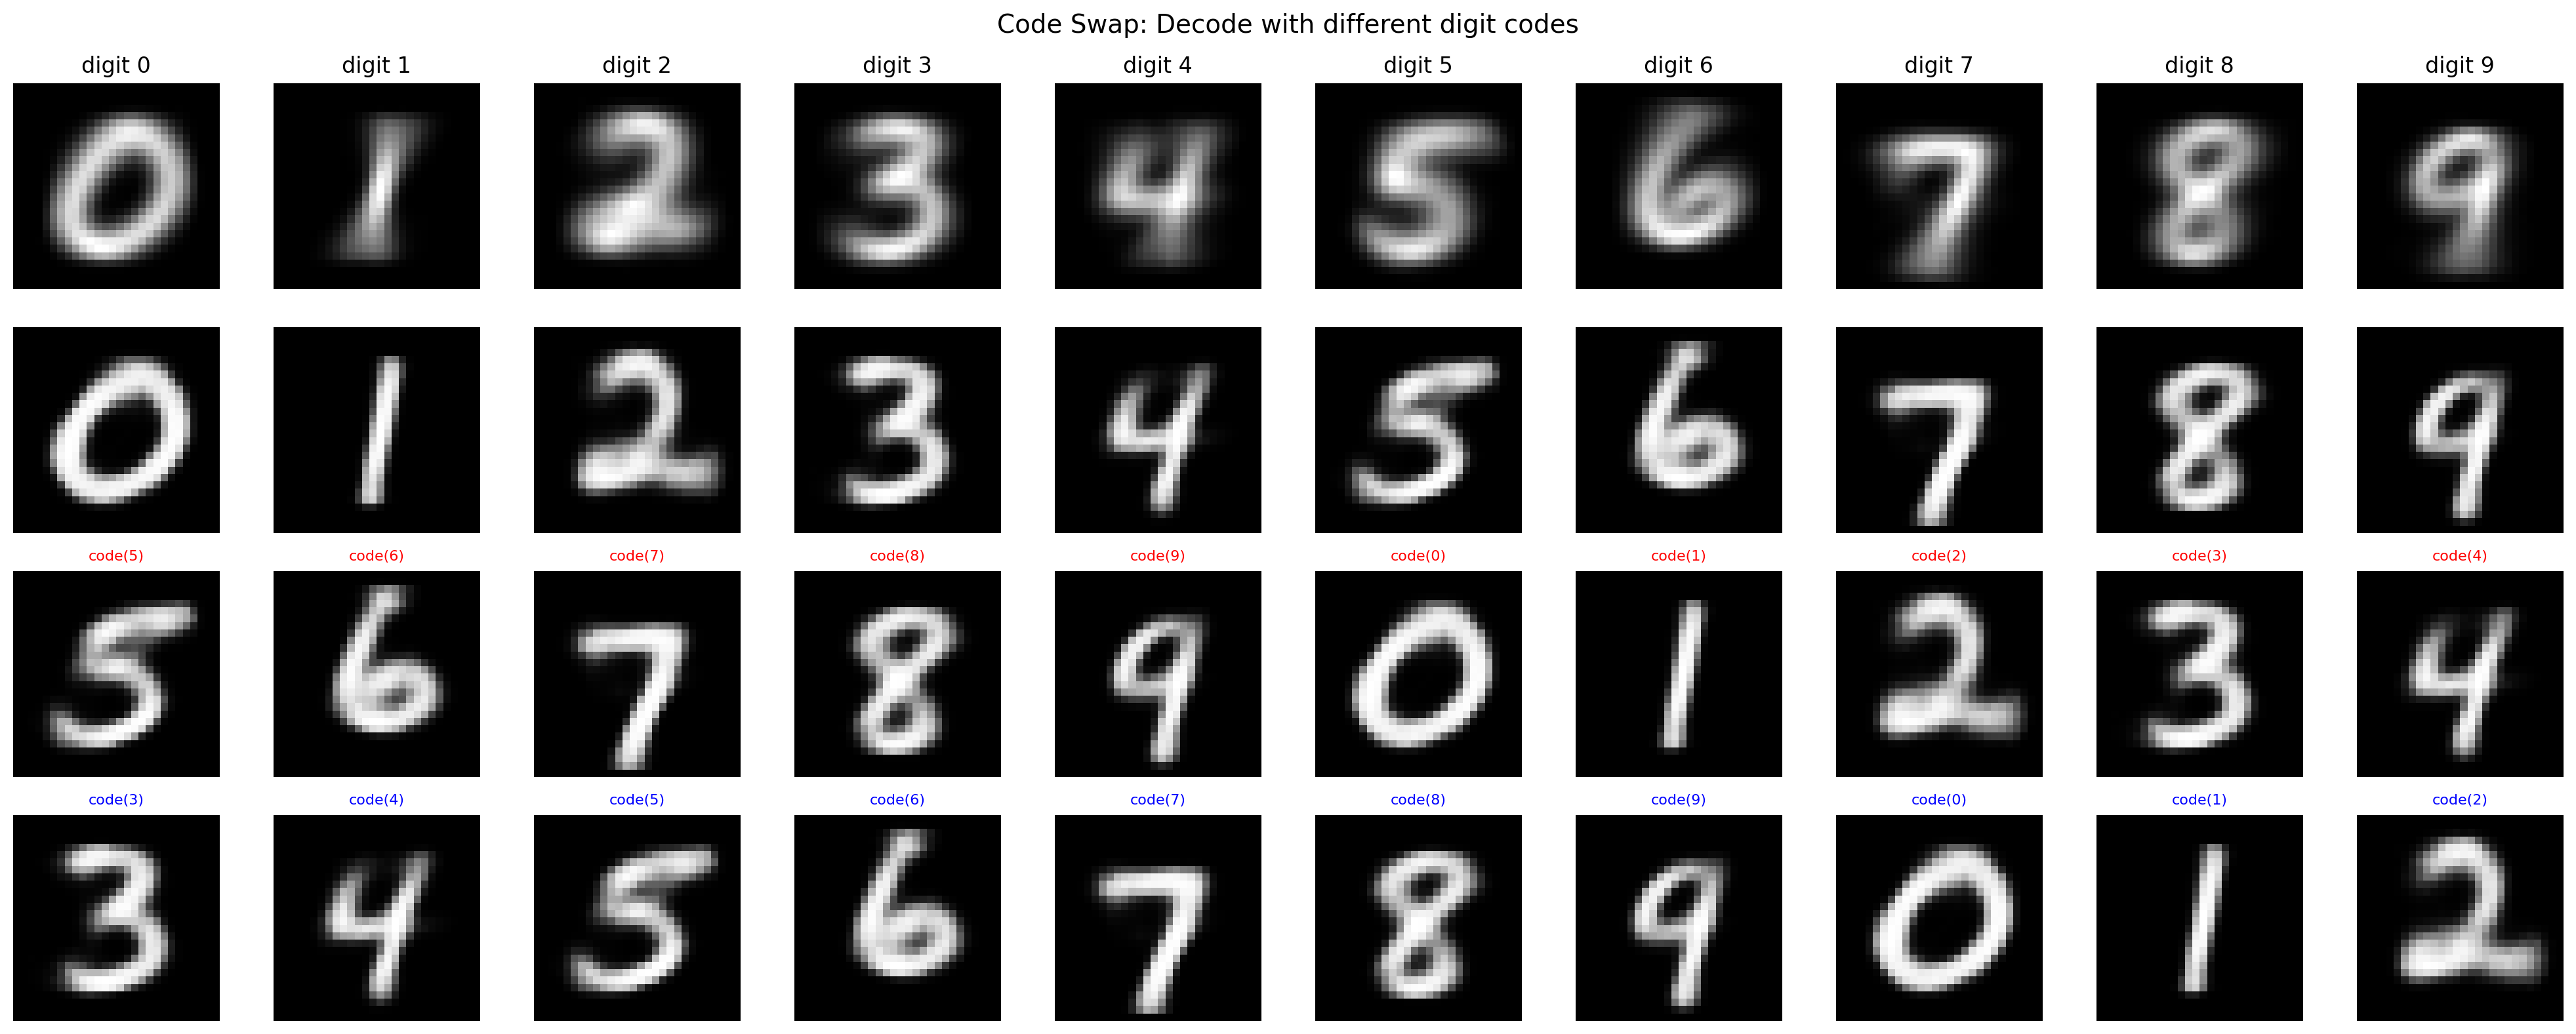
\includegraphics[width=0.75\columnwidth]{figures/code_swap.png}
\caption{MNIST code swap causality test. Decoding with digit $X$'s 32-bit code always produces digit $X$'s reconstruction, regardless of the input image. The discrete code fully determines the output.}
\label{fig:code_swap}
\end{figure}


\subsection{Pythia-70M Sparse Autoencoder}

\textbf{Setup.} We used EleutherAI's pre-trained sparse autoencoder (\texttt{sae-pythia-70m-32k}) on layer~3 MLP outputs of Pythia-70M~\citep{biderman2023pythia}. We defined 60 probe concepts across 6 semantic domains (physical, animals, emotions, abstract, social, properties) and tracked 256 SAE features (selected by activation frequency at the final checkpoint) across 12 training checkpoints from step~1 to step~143{,}000.

\textbf{Lifecycle.} reptimeline detected 1{,}835 births, 875 deaths, and 1{,}770 connections, with 2 phase transitions detected automatically. 64 of 256 tracked features were active (the remaining 192 were effectively dead---expected given SAE sparsity).

\textbf{Discovery.} BitDiscovery found 34 dual pairs, 227 dependency edges, and 74 three-way AND-gate interactions. Auto-labeling via embedding centroids produced interpretable names: ``teacher,'' ``belief,'' ``dog,'' ``wisdom,'' ``ocean.'' Figure~\ref{fig:swimlane} shows the swimlane heatmap for the first 20 features across 12 checkpoints.

\textbf{Causal verification.} We tested all 16 active features via \emph{SAE causal intervention}: for each feature, we encoded all 60 concepts' hidden states via the SAE, zeroed the target feature, decoded back to hidden-state space, and injected the modified state into the model via a forward hook at layer~3. We measured the KL divergence between original and modified next-token predictions.

\textbf{8/16} features showed \textbf{finite KL selectivity} averaging $26.8\times$ L2 (best: $98.4\times$ for ``fast''; ``teacher'' at $26.6\times$ disproportionately affected \emph{child, dog, wolf, queen}). The remaining 8 features showed zero cross-activation, which may reflect SAE sparsity (the feature never fires for non-labeled concepts) rather than proven causal selectivity; we report these groups separately. L1-norm ratios yield a lower mean of $19.5\times$ on the same features. Figure~\ref{fig:sae_causal} shows the selectivity heatmap.

\begin{figure}[h]
\centering
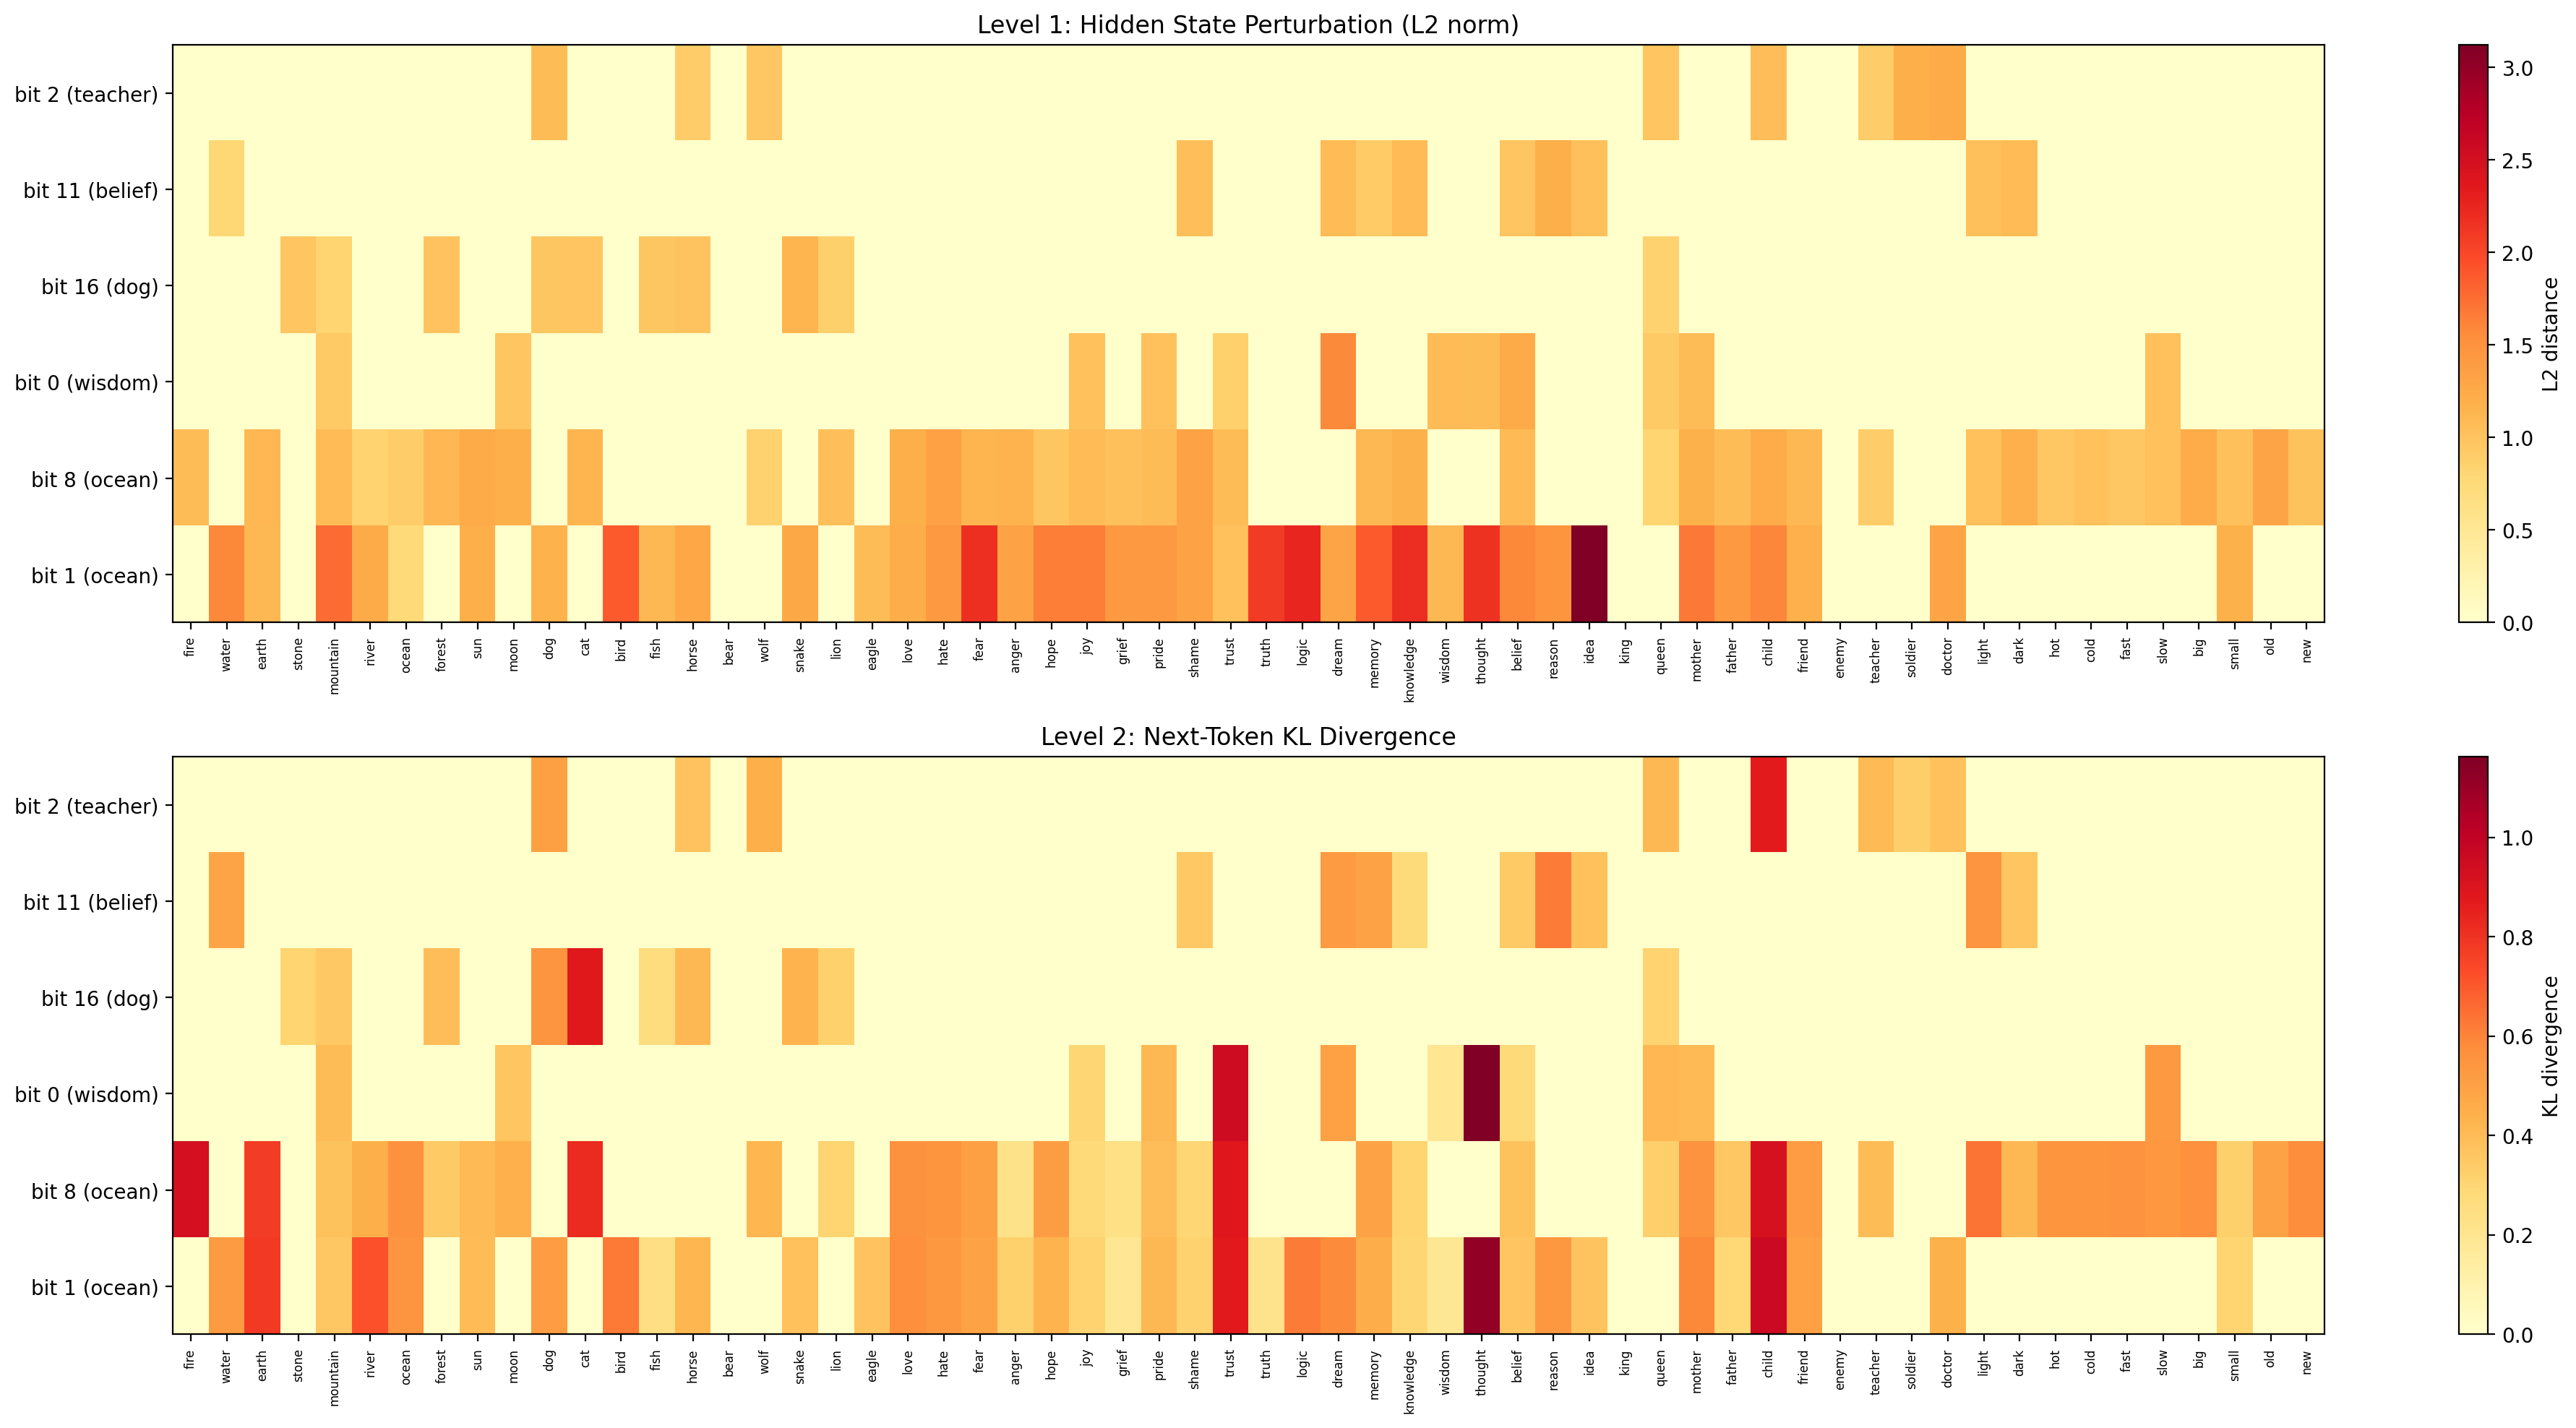
\includegraphics[width=\columnwidth]{figures/sae_intervention_heatmap.png}
\caption{Causal intervention on Pythia-70M SAE features (16 tested). \textbf{Top}: hidden state perturbation (L2 norm). \textbf{Bottom}: KL divergence in next-token predictions. Eight features are perfectly selective (only affect labeled concepts); the remaining eight average $26.8\times$ selectivity. ``fast'' (bit~14): $98.4\times$; ``teacher'' (bit~2): $26.6\times$. Yellow = no effect; dark red = strong effect.}
\label{fig:sae_causal}
\end{figure}

\begin{figure}[h]
\centering
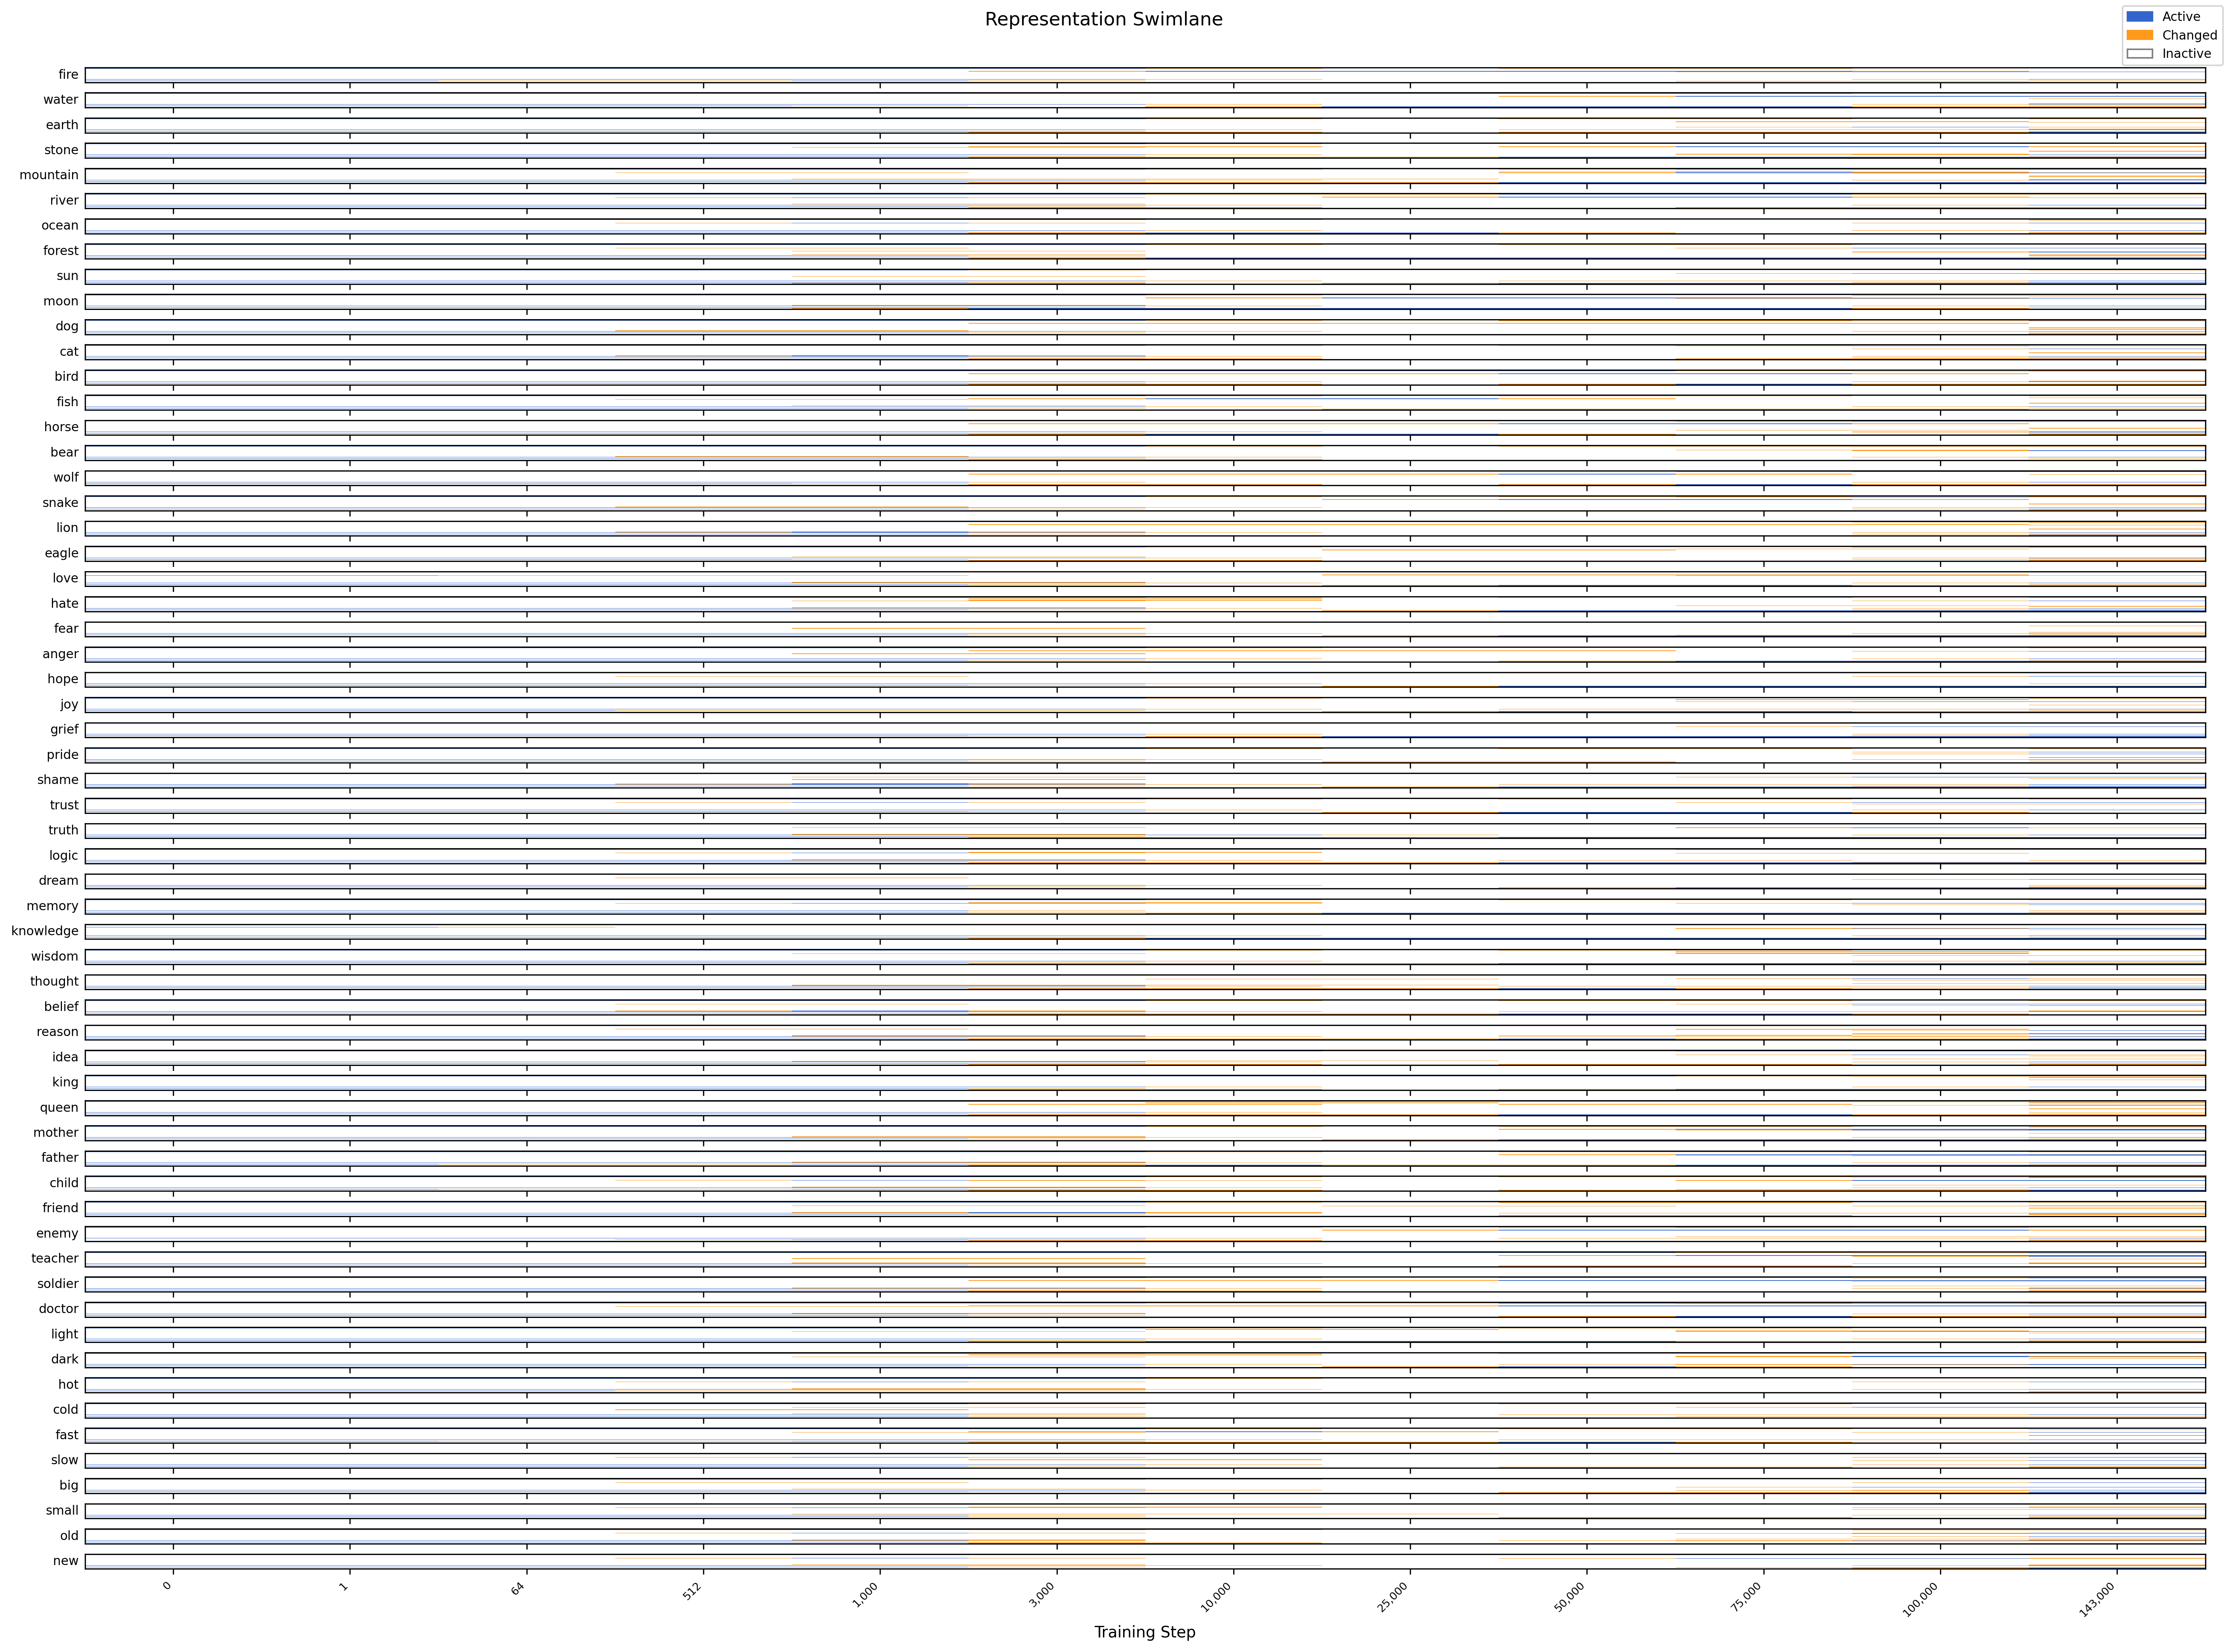
\includegraphics[width=\columnwidth]{figures/swimlane.png}
\caption{Swimlane visualization for Pythia-70M SAE features. Each row is a probe concept, each column a training checkpoint. Cell color indicates bit activation state: blue = active, white = inactive, orange = changed from previous step. The visualization reveals which concepts acquire or lose features over training and how representation structure crystallizes.}
\label{fig:swimlane}
\end{figure}


\subsection{TriadicGPT (63-bit Neurosymbolic Head)}

\textbf{Setup.} TriadicGPT~\citep{ornelas2026microgpt} is a 40M-parameter GPT that jointly learns next-token prediction and 63-bit discrete semantic projections via a triadic head trained end-to-end. reptimeline tracked 53 concepts across 8 checkpoints from step~2{,}500 to step~50{,}000.

\textbf{Lifecycle and phase discovery.} reptimeline revealed a \emph{four-phase training dynamic} invisible to standard scalar logging:
\begin{enumerate}[nosep]
    \item \textbf{Exploration} (steps 0--7{,}500): high bit churn across all concepts.
    \item \textbf{Consolidation} (7{,}500--27{,}500): churn remains elevated but entropy stabilizes.
    \item \textbf{Crystallization} ($\sim$27{,}500): entropy drops from 0.50 to 0.23 and utilization drops from 0.98 to 0.66 simultaneously---a sharp phase transition.
    \item \textbf{Stabilization} (27{,}500--50{,}000): churn collapses to 0.075; representations freeze.
\end{enumerate}

The crystallization event---the moment the model ``commits'' to its semantic assignments---is not visible in loss curves or standard metrics. Related crystallization phenomena have been studied in grokking~\citep{power2022grokking,nanda2023progress} and VQ-VAE codebook dynamics, but to our knowledge reptimeline is the first tool to detect such transitions automatically via per-code temporal analysis.

\textbf{Structural causality.} Unlike MNIST and Pythia where features lie in the computation path, TriadicGPT's triadic head is a parallel projection---flipping a bit direction in hidden space changes LM output (mean KL $> 0$) but not selectively (1/24 bits above $1.5\times$). This is an expected architectural consequence, not a tool limitation. The causality evidence for TriadicGPT is \emph{structural}: reptimeline discovers 9 anti-correlated dual pairs (e.g., vida/muerte at $r = 0.91$, placer/dolor at $r = 1.00$) that match the gold semantic axes defined in the training ontology, confirming that the model learned the intended semantic structure.

\textbf{Overlay analysis.} The \texttt{PrimitiveOverlay} module loaded the manually-defined ontology specifying 63 named primitives with layer assignments, dependency edges, and dual pairs. It computed four diagnostics:
(i)~\emph{activation epochs}---the first step each primitive activates per concept;
(ii)~\emph{dependency completions}---when all required dependencies are simultaneously active;
(iii)~\emph{layer emergence}---aggregate statistics per layer (earliest, median, latest activation step);
(iv)~\emph{dual coherence}---whether anti-correlated pairs exhibit exclusive activation, scored as $n_{\text{excl}} / (n_{\text{excl}} {+} n_{\text{both}})$.
Layer emergence confirmed that lower-layer primitives (structural) stabilized before higher-layer ones (semantic), consistent with the expected hierarchy.

\textbf{Reconciliation.} The Reconciler achieved 44.4\% agreement between model-discovered and manually-defined ontology, identifying 35 critical mismatches (including 8 \emph{dead\_but\_assigned} and 12 \emph{active\_but\_unassigned} bits) that guided anchor expansion from 50 to 158 concepts in subsequent training iterations. The Reconciler produced correction suggestions for both directions: 5 anchor retraining recommendations and 8 theory update suggestions.

\begin{figure}[h]
\centering
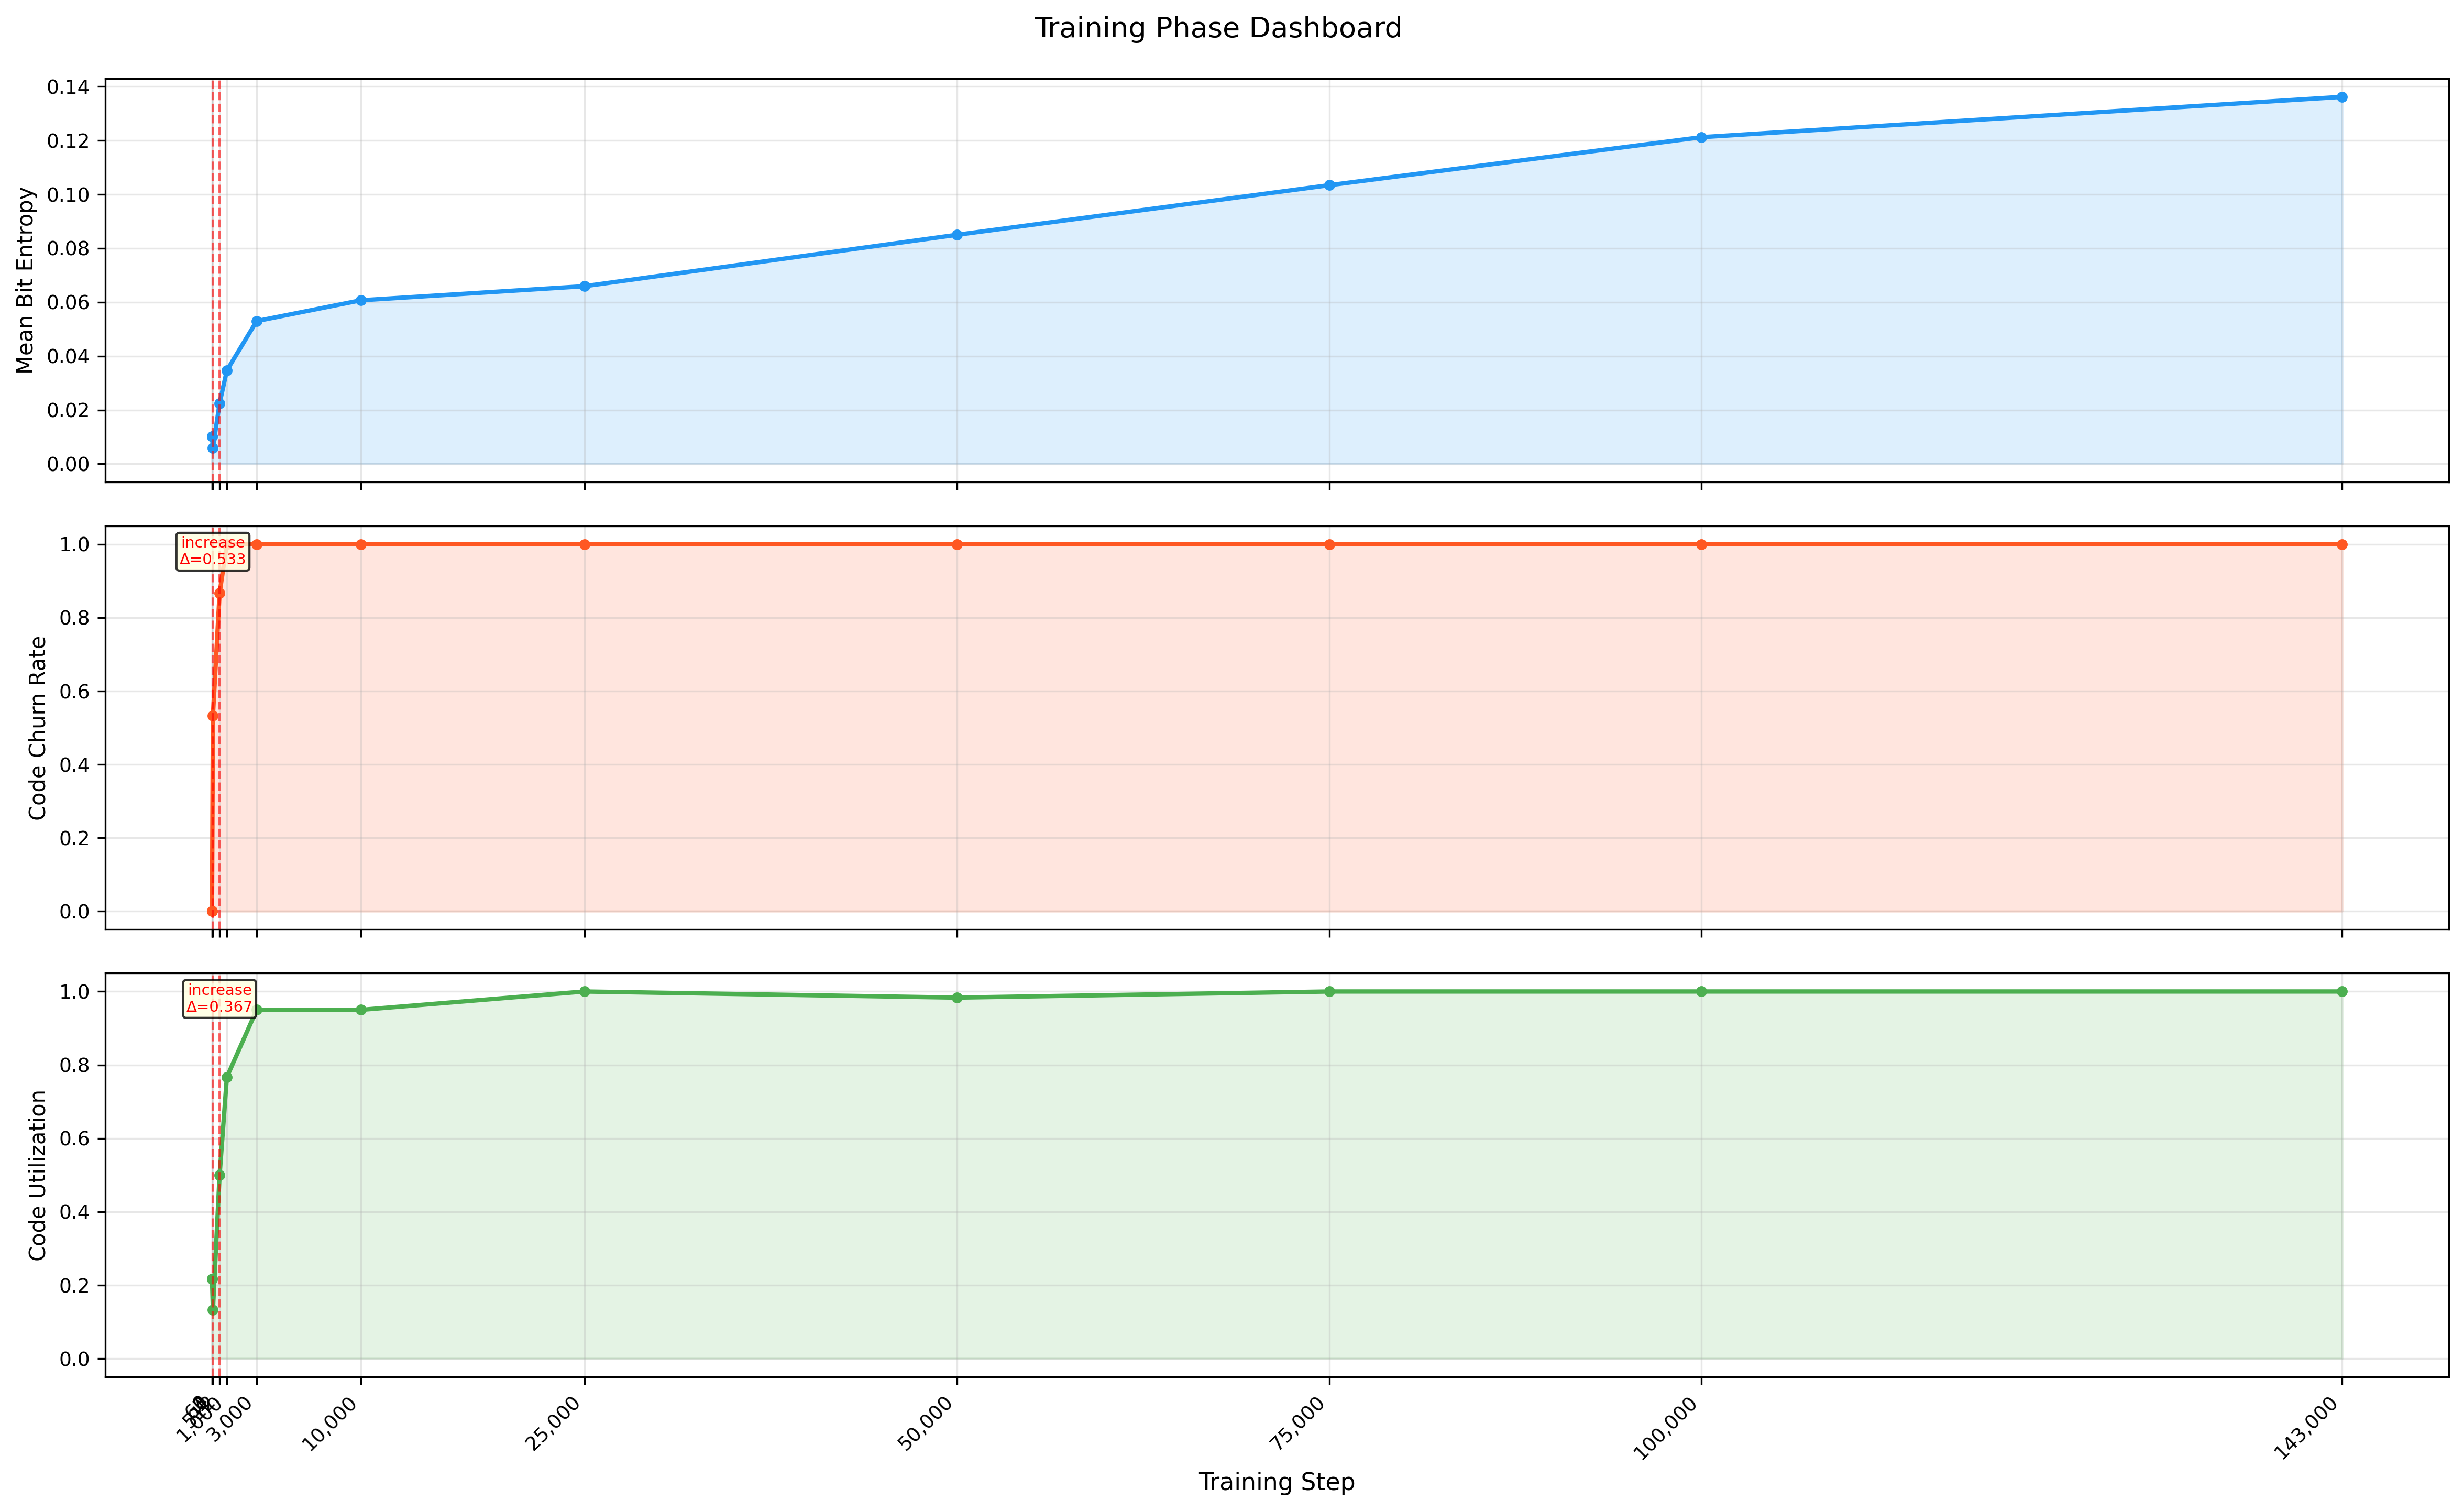
\includegraphics[width=\columnwidth]{figures/phase_dashboard.png}
\caption{Pythia-70M phase dashboard: entropy, churn rate, and utilization curves across 12 training checkpoints. Vertical lines mark automatically detected phase transitions. Similar four-phase dynamics were observed in TriadicGPT training.}
\label{fig:phase}
\end{figure}


\subsection{Prediction Experiment: Negative Results}

We tested whether the 8 finite-selectivity SAE features could improve next-token prediction. Two strategies were evaluated: (1)~embedding-based feature selection from the discovered set; (2)~MLP-based prediction using feature activations. Neither improved over the unmodified Pythia-70M baseline: embedding-based achieved $-0.13\%$ relative accuracy, and MLP-based achieved $-4.20\%$. The individual features are causally meaningful (removing them selectively changes predictions) but combining them for prediction does not yet yield improvements. This suggests that selective causal influence is necessary but not sufficient for useful feature-based prediction.


% ============================================================
\section{Comparison with Existing Tools}
\label{sec:comparison}
% ============================================================

Table~\ref{tab:comparison} compares reptimeline with existing approaches for monitoring and interpreting discrete representations.

\begin{table}[h]
\centering
\caption{Feature comparison across discrete representation tools. \checkmark\ = full support, Partial = aggregate only, Manual = requires human effort, --- = not supported.}
\label{tab:comparison}
\small
\begin{tabular}{lccccc}
\toprule
Capability & \textbf{reptimeline} & VQ-VAE & SAE & CBM & RepE \\
\midrule
Per-code lifecycle & \checkmark & Partial & Partial & --- & --- \\
Connection tracking & \checkmark & --- & --- & --- & --- \\
Phase transition detection & \checkmark & --- & Manual & --- & --- \\
3-way interaction discovery & \checkmark & --- & --- & --- & --- \\
Bottom-up ontology discovery & \checkmark & --- & --- & --- & --- \\
Auto-labeling (3 strategies) & \checkmark & --- & Manual & Manual & --- \\
Causal verification (stat.) & \checkmark & --- & --- & --- & \checkmark \\
Multiple-comparison correction & \checkmark & --- & --- & --- & --- \\
Built-in extractors & \checkmark\ (3) & --- & --- & --- & --- \\
JSON/CSV export & \checkmark & --- & Partial & --- & --- \\
Backend-agnostic & \checkmark & --- & --- & --- & --- \\
\bottomrule
\end{tabular}
\end{table}

\textbf{VQ-VAE tools} (e.g., WandB codebook metrics) track aggregate utilization and commitment loss but not per-code lifecycle events. \textbf{SAE dashboards} (e.g., Neuronpedia~\citep{bricken2023monosemanticity,templeton2024scaling}) provide manual feature browsing for sparse autoencoders but are architecture-specific and do not track temporal evolution. Recent work on automated circuit discovery~\citep{conmy2023automated} identifies computational circuits but does not track discrete code evolution. The superposition hypothesis~\citep{elhage2022superposition} motivates SAE-based feature extraction; reptimeline operates downstream, analyzing the features SAEs produce. \textbf{Concept Bottleneck Model (CBM) tools}~\citep{koh2020concept} require predefined concept annotations and do not discover structure bottom-up. \textbf{Representation Engineering (RepE)}~\citep{zou2023representation} identifies directions in continuous space but does not operate on discrete codes.

reptimeline differs fundamentally: it operates on the discrete codes themselves, requires no predefined labels, discovers structure bottom-up, and verifies causality---all through a single backend-agnostic API.

\noindent\textit{Note:} Table~\ref{tab:comparison} compares tool categories rather than specific implementations. Individual tools within each category may offer partial overlapping capabilities not captured by a binary comparison.


% ============================================================
\section{Conclusion and Availability}
\label{sec:conclusion}
% ============================================================

reptimeline fills a gap in the discrete representation toolbox. It reveals training dynamics that scalar logging misses (crystallization events), discovers interpretable structure without supervision (duals, dependencies, three-way interactions), and verifies that discovered features are causally meaningful---with rigorous statistical methodology including bootstrap confidence intervals, permutation tests, Benjamini-Hochberg FDR correction, and Cohen's $d$ effect sizes (8/16 with finite KL selectivity at 26.8$\times$ mean on Pythia-70M, 100\% decoder determinism on MNIST).

\textbf{Availability.} \texttt{pip install reptimeline}. Source code, examples, and pre-computed results are available at \url{https://github.com/arturoornelasb/reptimeline}. Licensed under BUSL-1.1 (free for research; converts to AGPL-3.0 in 2030). The package includes 224~unit tests at 92\% coverage, 11~example pipelines, 6~visualization modules (5~static, 4~interactive), 3~built-in extractors (VQ-VAE, SAE, FSQ), JSON/CSV export, a command-line interface, and a structured exception hierarchy. All statistical methods are implemented in pure NumPy with no SciPy dependency.

\textbf{Future work.} (1)~Streaming mode for real-time monitoring during training. (2)~Integration with WandB/TensorBoard as a plugin. (3)~Extension to continuous representations via learned discretization. (4)~Active learning loop: use Reconciler mismatches to automatically suggest retraining targets.


% ============================================================
% References
% ============================================================

\bibliographystyle{plainnat}

\begin{thebibliography}{10}

\bibitem[Bengio et~al.(2013)]{bengio2013estimating}
Y.~Bengio, N.~L\'{e}onard, and A.~Courville.
\newblock Estimating or propagating gradients through stochastic neurons for conditional computation.
\newblock \emph{arXiv preprint arXiv:1308.3432}, 2013.

\bibitem[Biderman et~al.(2023)]{biderman2023pythia}
S.~Biderman, H.~Schoelkopf, Q.~Anthony, H.~Bradley, K.~O'Brien, E.~Hallahan, M.~A. Khan, S.~Purohit, U.~S. Prashanth, E.~Raff, et~al.
\newblock Pythia: A suite for analyzing large language models across training and scaling.
\newblock In \emph{ICML}, 2023.

\bibitem[Cunningham et~al.(2023)]{cunningham2023sparse}
H.~Cunningham, A.~Ewart, L.~Riggs, R.~Huben, and L.~Sharkey.
\newblock Sparse autoencoders find highly interpretable features in language models.
\newblock \emph{arXiv preprint arXiv:2309.08600}, 2023.

\bibitem[Koh et~al.(2020)]{koh2020concept}
P.~W. Koh, T.~Nguyen, Y.~S. Tang, S.~Mussmann, E.~Pierson, B.~Kim, and P.~Liang.
\newblock Concept bottleneck models.
\newblock In \emph{ICML}, 2020.

\bibitem[Mentzer et~al.(2024)]{mentzer2024finite}
F.~Mentzer, D.~Minnen, E.~Agustsson, and M.~Tschannen.
\newblock Finite scalar quantization: {VQ-VAE} made simple.
\newblock In \emph{ICLR}, 2024.

\bibitem[Power et~al.(2022)]{power2022grokking}
A.~Power, Y.~Burda, H.~Edwards, I.~Babuschkin, and V.~Misra.
\newblock Grokking: Generalization beyond overfitting on small algorithmic datasets.
\newblock In \emph{ICLR Workshop}, 2022.

\bibitem[Ornelas~Brand(2026a)]{ornelas2026prime}
J.~A. Ornelas~Brand.
\newblock Prime factorization as a neurosymbolic bridge: Projecting continuous embeddings into discrete algebraic space for deterministic verification.
\newblock 2026.
\newblock \href{https://doi.org/10.5281/zenodo.19205805}{doi:10.5281/zenodo.19205805}.

\bibitem[Ornelas~Brand(2026b)]{ornelas2026microgpt}
J.~A. Ornelas~Brand.
\newblock End-to-end prime factorization in a generative language model: Emergent algebraic semantics from joint training.
\newblock 2026.
\newblock \href{https://doi.org/10.5281/zenodo.19206545}{doi:10.5281/zenodo.19206545}.

\bibitem[van~den Oord et~al.(2017)]{vandenoord2017neural}
A.~van~den Oord, O.~Vinyals, and K.~Kavukcuoglu.
\newblock Neural discrete representation learning.
\newblock In \emph{NeurIPS}, 2017.

\bibitem[Zou et~al.(2023)]{zou2023representation}
A.~Zou, L.~Phan, S.~Chen, J.~Campbell, P.~Guo, R.~Ren, A.~Pan, X.~Yin, M.~Mazeika, A.~Dombrowski, et~al.
\newblock Representation engineering: A top-down approach to {AI} transparency.
\newblock \emph{arXiv preprint arXiv:2310.01405}, 2023.

\bibitem[Nanda et~al.(2023)]{nanda2023progress}
N.~Nanda, L.~Chan, T.~Lieberum, J.~Smith, and J.~Steinhardt.
\newblock Progress measures for grokking via mechanistic interpretability.
\newblock In \emph{ICLR}, 2023.

\bibitem[Bricken et~al.(2023)]{bricken2023monosemanticity}
T.~Bricken, A.~Templeton, J.~Batson, B.~Chen, A.~Jermyn, T.~Conerly, N.~Turner, C.~Anil, C.~Denison, A.~Askell, et~al.
\newblock Towards monosemanticity: Decomposing language models with dictionary learning.
\newblock \emph{Transformer Circuits Thread}, Anthropic, 2023.

\bibitem[Sharkey et~al.(2022)]{sharkey2022taking}
L.~Sharkey, D.~Braun, and B.~Millidge.
\newblock Taking features out of superposition with sparse autoencoders.
\newblock \emph{arXiv preprint arXiv:2211.11279}, 2022.

\bibitem[Conmy et~al.(2023)]{conmy2023automated}
A.~Conmy, A.~N. Mavor-Parker, A.~Lynch, S.~Heimersheim, and A.~Garriga-Alonso.
\newblock Towards automated circuit discovery for mechanistic interpretability.
\newblock In \emph{NeurIPS}, 2023.

\bibitem[Elhage et~al.(2022)]{elhage2022superposition}
N.~Elhage, T.~Hume, C.~Olsson, N.~Schiefer, T.~Henighan, S.~Kravec, Z.~Hatfield-Dodds, R.~Lasenby, D.~Drain, C.~Chen, et~al.
\newblock Toy models of superposition.
\newblock \emph{Transformer Circuits Thread}, Anthropic, 2022.

\bibitem[Templeton et~al.(2024)]{templeton2024scaling}
A.~Templeton, T.~Conerly, J.~Marcus, J.~Lindsey, T.~Bricken, B.~Chen, A.~Pearce, C.~Citro, E.~Ameisen, A.~Jones, et~al.
\newblock Scaling monosemanticity: Extracting interpretable features from {Claude} 3 {Sonnet}.
\newblock \emph{Transformer Circuits Thread}, Anthropic, 2024.

\end{thebibliography}

\end{document}
